\section{Deployment Diagram}
The system is designed to take two images of splints and output the comparison result. In order to obtain a photo of the splint a camera is used, that captures the alignment of the lines on the surface of the split, then that image is being passed to the program that performs the recognition and comparison process.
\begin{figure}[h]
	\centering
	
\includegraphics[width=\textwidth]{images/deployment_diagram}
	\caption{Deployment Diagram}
\end{figure}

\section{Image Acquisition}
\paragraph{}
Images used while developing the program were shot on a regular iPhone. Also the light conditions were far from ideal. Plenty of images contain either light reflexes or extensive shades. Moreover, image background and surroundings differ which makes the processing more error prone (see figure \ref{fig:different_lightning_conditions}).

\begin{figure}[H]
     \centering
     \subfloat[]{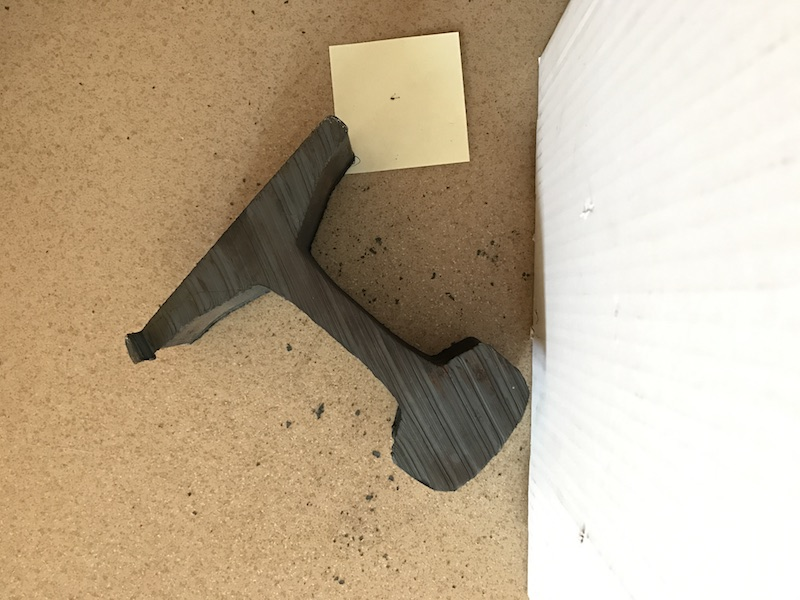
\includegraphics[width=0.45\textwidth]{images/example_splint}}
     \qquad
     \subfloat[]{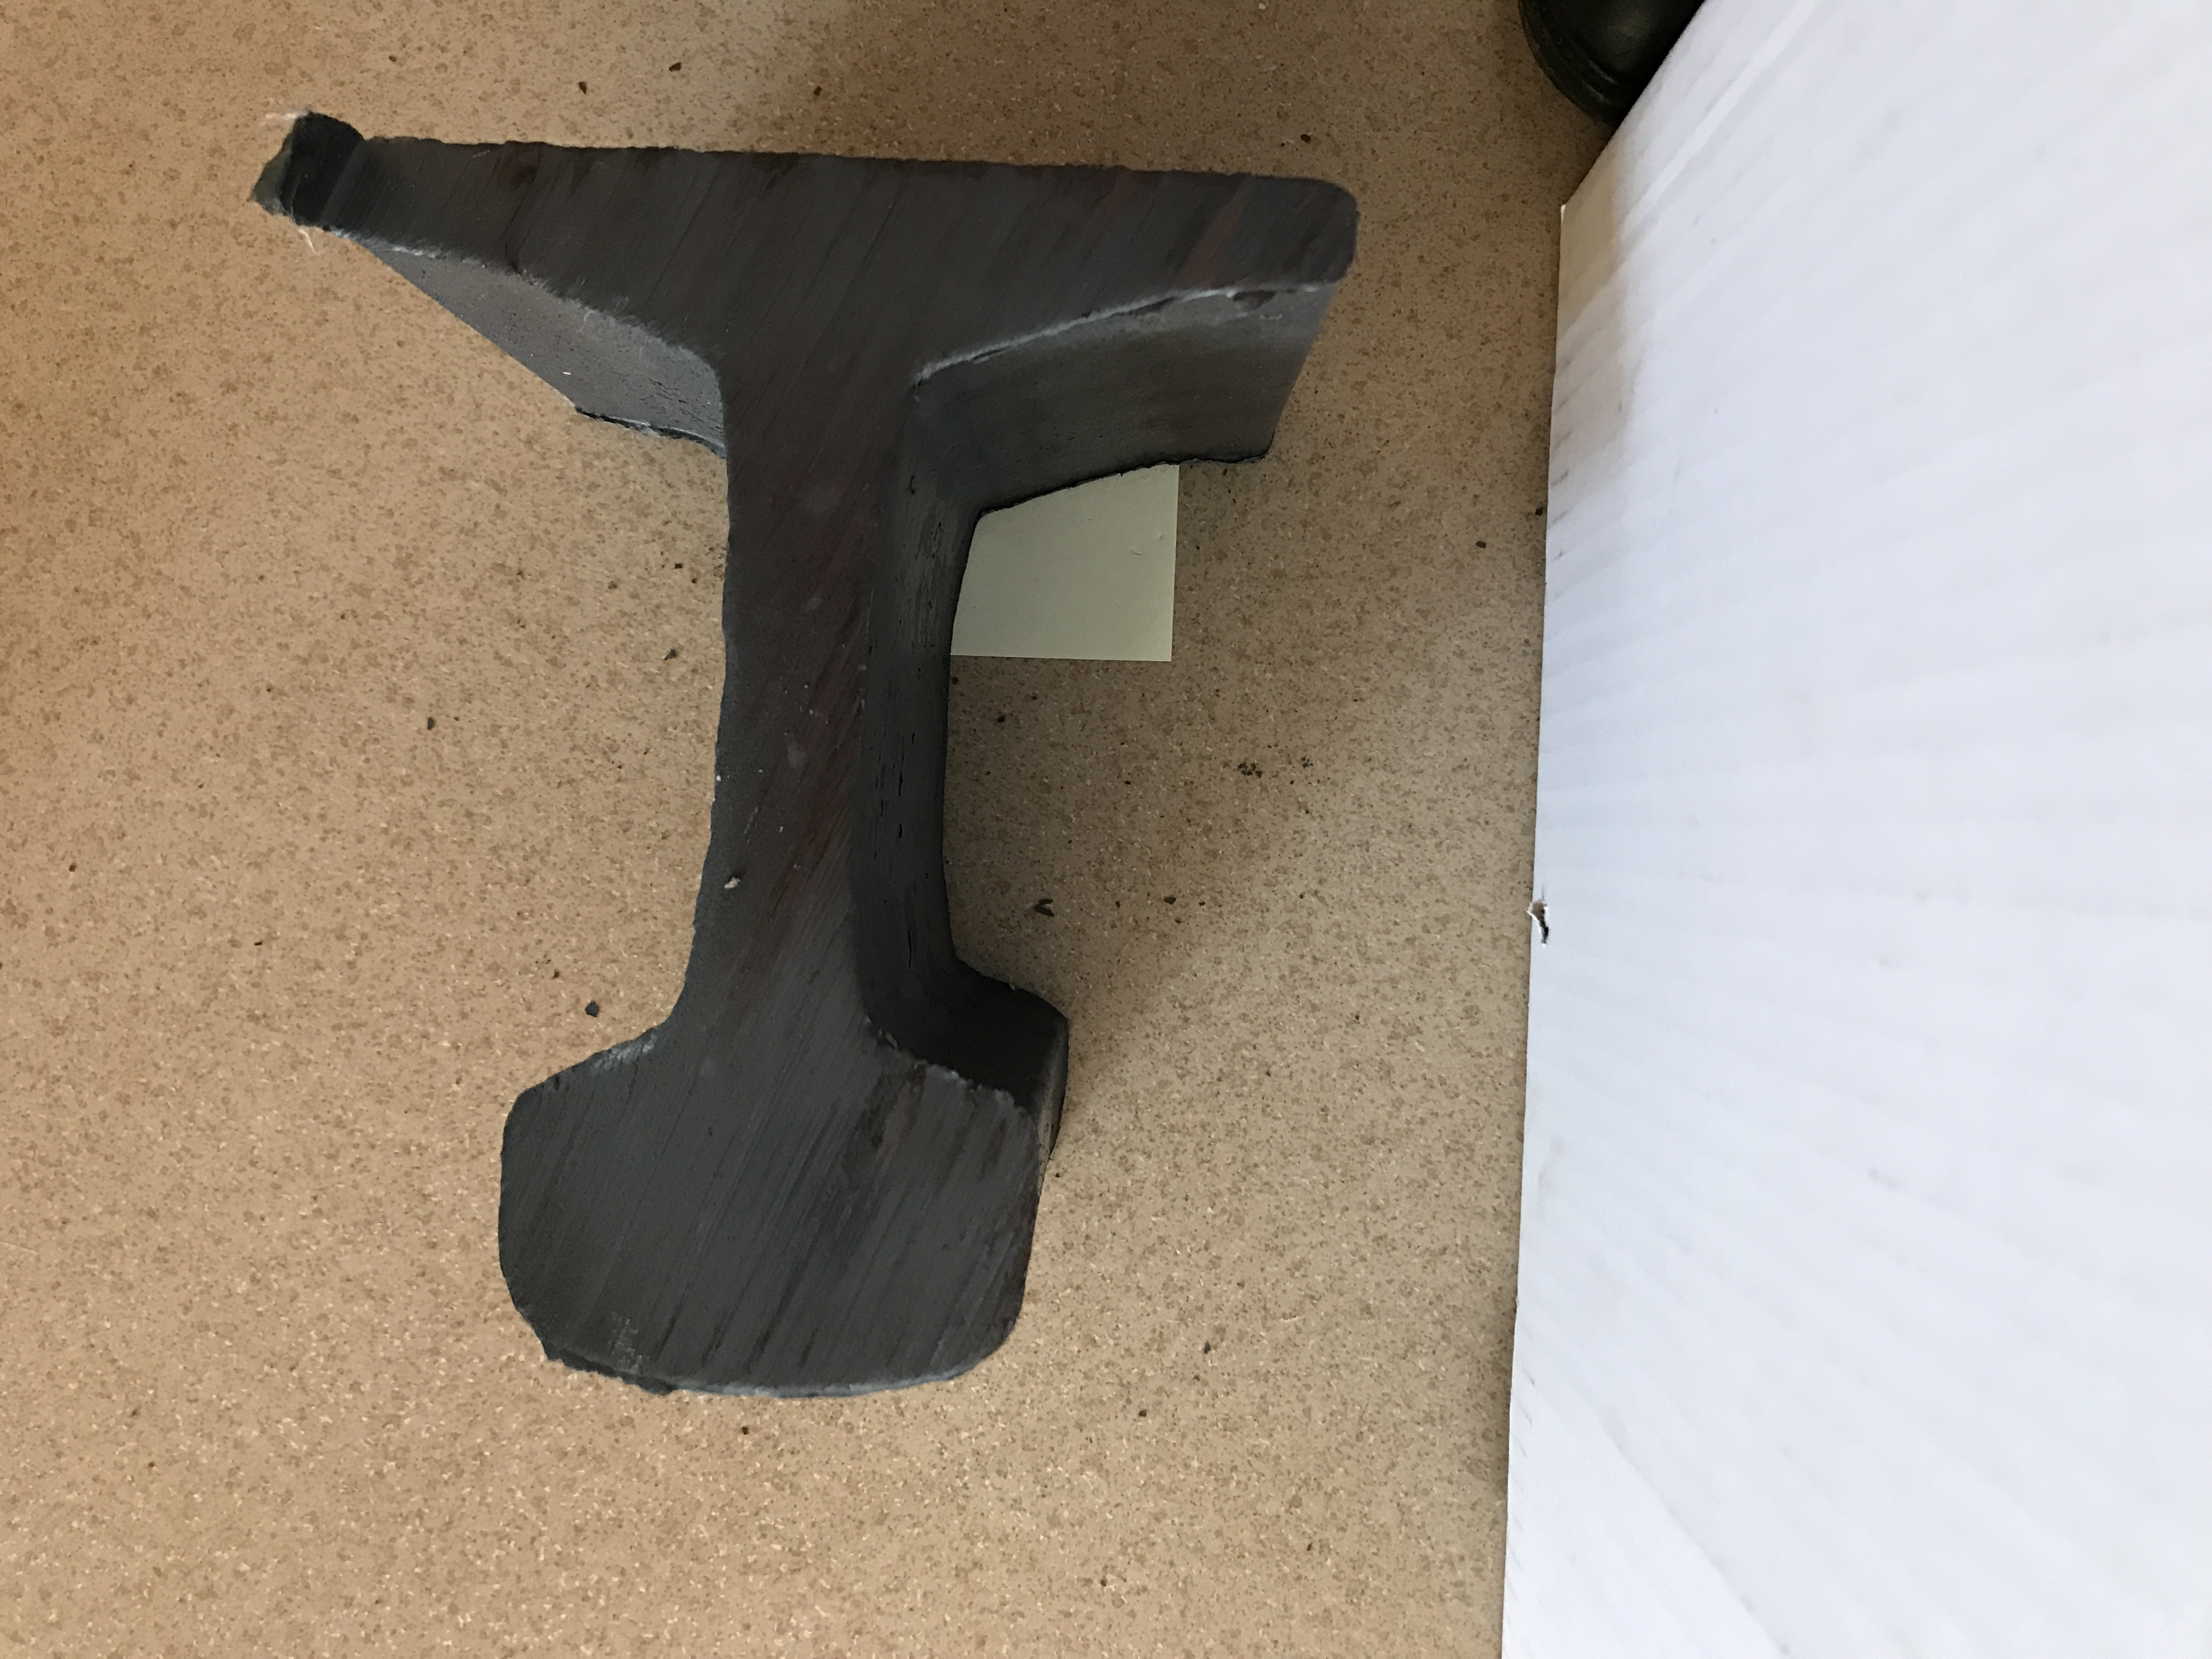
\includegraphics[width=0.45\textwidth]{images/example_splint_2}}
     \qquad
     \vfill
     \subfloat[]{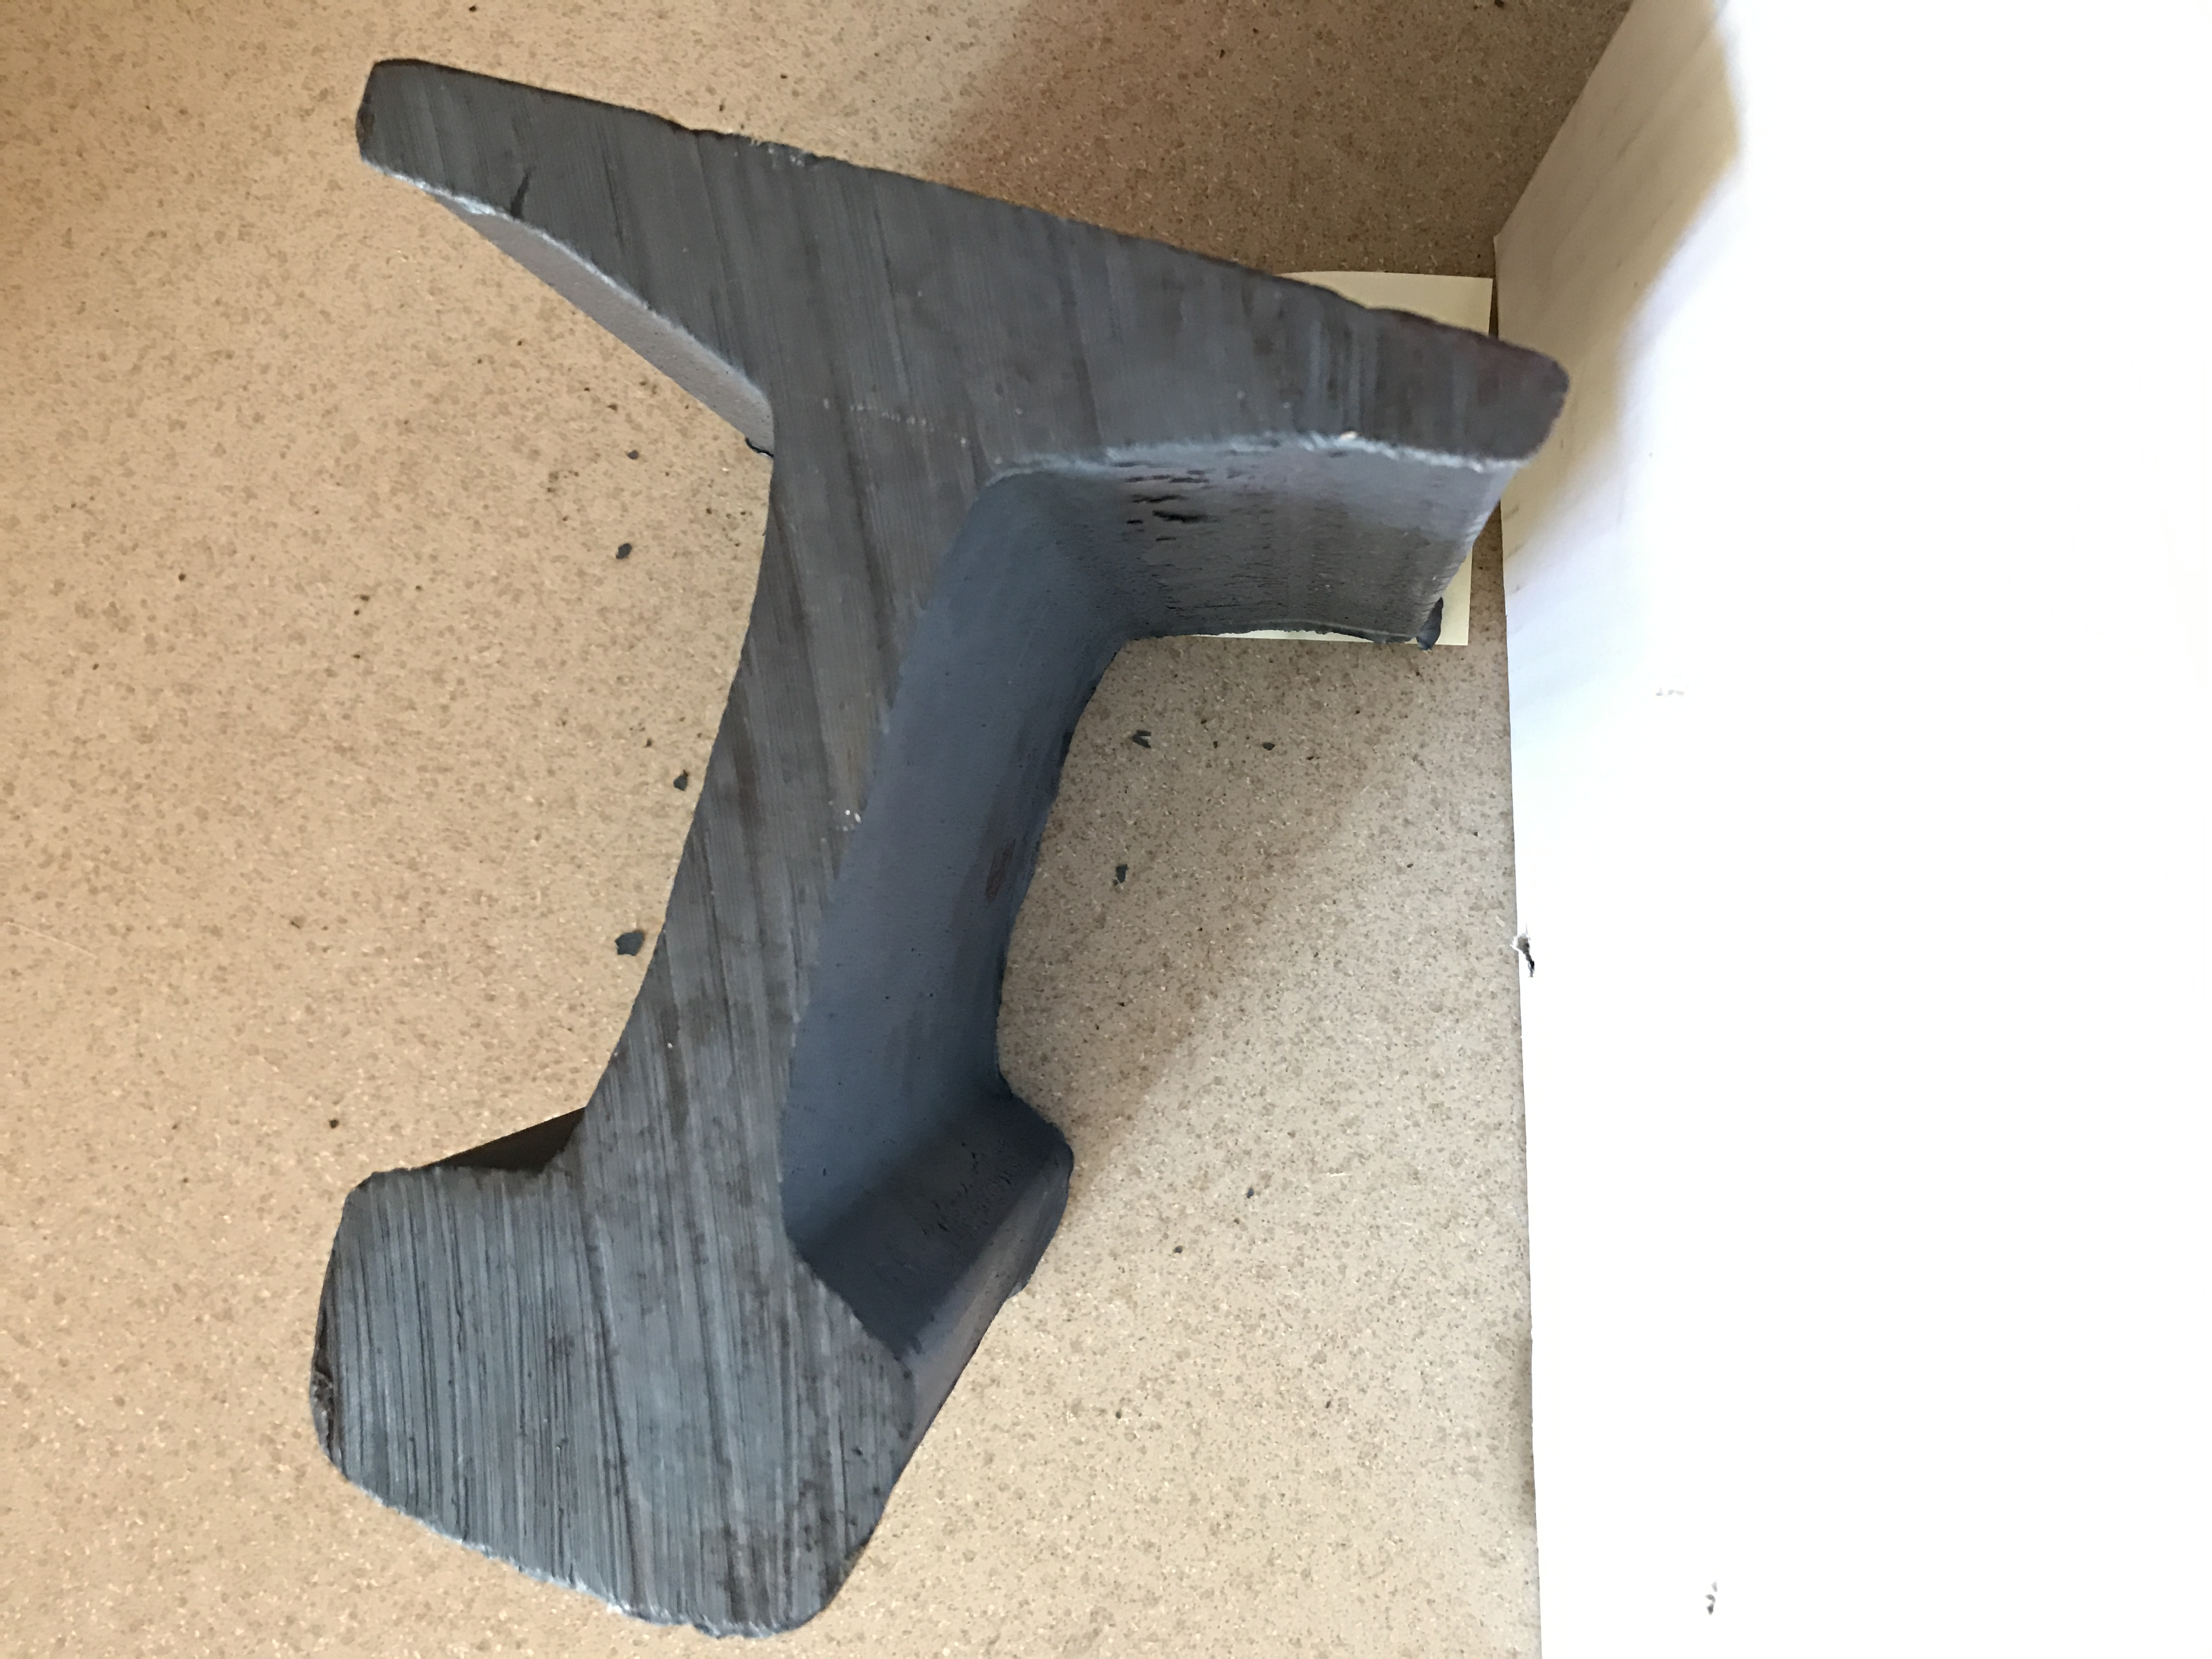
\includegraphics[width=0.45\textwidth]{images/example_splint_3}}
     \qquad
     \subfloat[]{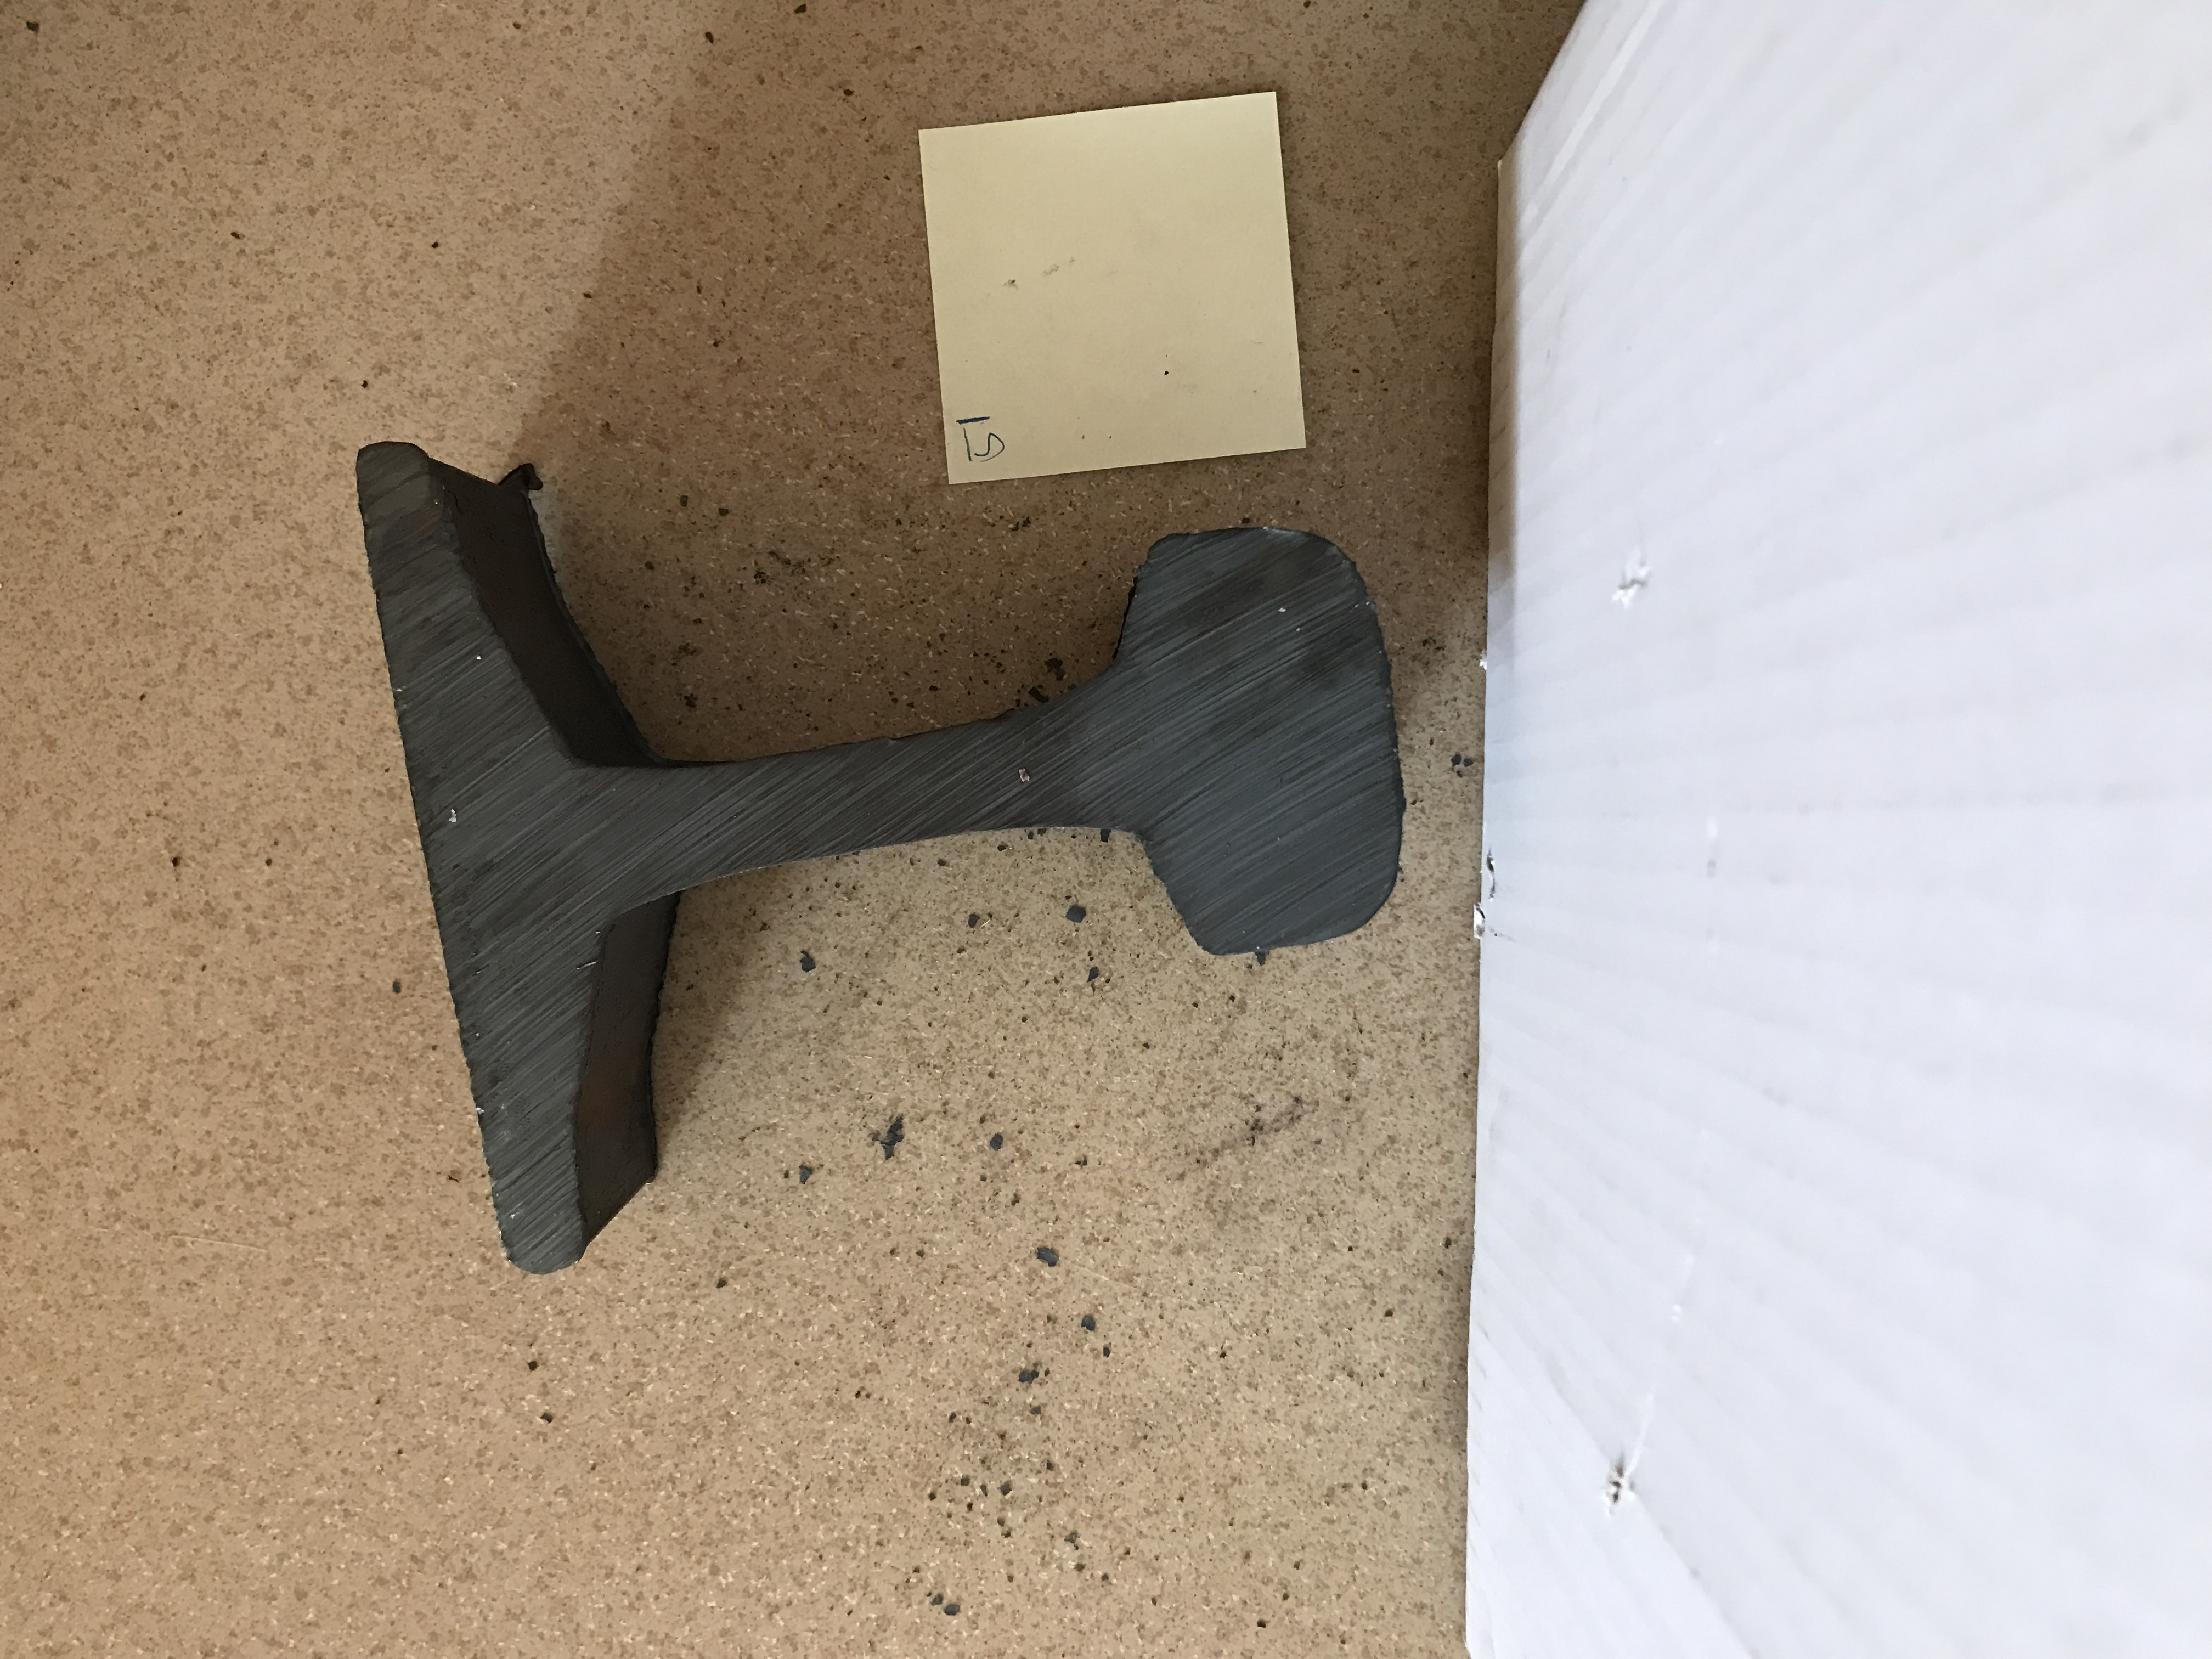
\includegraphics[width=0.45\textwidth]{images/example_splint_4}}
     \caption{Sample images of splints}
     \label{fig:different_lightning_conditions}
\end{figure}
 
\paragraph{}
However, provided the system will be implemented in production use, professional equipment will be installed (for example high quality camera) and maximal effort will be undertaken to ensure similar light conditions and background (ideally striking, monochromatic colour)

\section{Image Preprocessing}
\paragraph{Note}
The preprocessing of the image in our case means extracting from the input image just the parts that we are interested in and dropping the rest. Specifically, the only part of the splint that is of interest to us is the surface. So the desired output of this phase is an image containing only the surface of the splint with everything else as mono-coloured background (for example white). This is not the main focus of this thesis, so only a simplified, although giving very promising results, approach will be shown. It is likely that fine-tuning this algorithm would lead to having a fully working preprocessing stage.

\paragraph{Initial algorithm}
Before computing the "barcode" representation of the splint there is a couple of steps required to enable processing. The primary goal is to extract the shape of the split from the image, effectively ignoring everything else. Let us now look at the first attempt to approach this task using following techniques:

\begin{enumerate}
	\item Image thresholding (binary) - it is a function that for a given grayscale pixel assigns one of two values {A, B}. A is assigned to all of the pixels with value greater than some threshold value and B otherwise.
	$$
	threshold (pixel, T) = \begin{cases}
		A, pixel.value > T \\
		B, pixel.value <= T
	\end{cases}
	$$
	\item Finding contours - a function finding curves joining continuous points, having same colour or intensity
\end{enumerate}

\begin{algorithm}{\textbf{Extracting the shape of the split - first approach}}
	\begin{spacing}{1.5}
	\begin{algorithmic}[1]
		\Function{extract}{$grayscale$}
			\State $threshold \gets \textbf{cv2.threshold}(grayscale)$
			\State $contours \gets \textbf{cv2.findContours}(threshold)$
			\State $splintContour \gets \textbf{maxArea}(contours)$
			\State $mask \gets \textbf{createMask}(splintContour)$
			\State \textbf{return} $\textbf{cropImage}(grayscale, mask)$
		\EndFunction
	\end{algorithmic}
	\end{spacing}
\end{algorithm}

The pseudocode presented above greatly simplifies the usage of OpenCV library. It does not provide any of the other required parameters for library functions and it also discards other return values. Function steps provide just the essential parts of the algorithm to present the idea. Regarding abstract functions, please ignore implementation details and just note that:
\begin{enumerate}
	\item \textbf{maxArea()} - finds the contour with maximal area amongst ones provided as the parameter
	\item \textbf{createMask()} - creates a mask that includes the whole shape of contour (i.e. the edge and the interior) for a given contour
	\item \textbf{cropImage()} - to a given image applies a given mask, effectively cutting out just those pixels specified by the mask 
\end{enumerate}

\paragraph{Improved algorithm}
Further development of the preprocessing algorithm led to a little bit more complex series of steps. Instead of converting whole RGB image to grayscale, the multi-channel array is split into separate single-channel arrays. Empirical experiments showed that for the given set of input images best results can be obtained when using just the red colour channel. The thresholding phase is now executed with threshold value computed from the histogram (first, peak value that corresponds to the splint is found and then after performing simple algebraic operations is used to obtain the value). The thresholding process returns a binary image where white colour denotes area that is most likely a part of the splint and a black colour otherwise. Such a binary image then undergoes a series of corresponding image blurring (using median blur filter) and morphological opening (which is a series of erosions followed by dilations). To complete the process and fill some gaps that may have appeared in some of the previous phases, a fill holes procedure is applied.

\begin{algorithm}{\textbf{Extracting the shape of the split - improved approach}}
	\begin{spacing}{1.5}
	\begin{algorithmic}[1]
		\Function{extract}{$image$}
			\State $redChannel \gets$ R channel from the $image$
			\State $splintPeak \gets$ Splint peak from histogram of $redChannel$
			\State $threshold \gets \textbf{threshold}(redChannel, splintPeak)$
			\State $blur \gets \textbf{cv2.medianBlur}(threshold)$
			\For{$i \gets 0\ \textbf{to}\ repetitions$}
				\State $opening \gets \textbf{open}(blur)$
				\State $blur \gets \textbf{cv2.medianBlur}(opening)$
			\EndFor
			\State $filled \gets \textbf{fillHoles}(blur)$
			\State $contours \gets \textbf{cv2.findContours}(filled)$
			\State $splintContour \gets \textbf{maxArea}(contours)$
			\State $mask \gets \textbf{createMask}(splintContour)$
			\State \textbf{return} $\textbf{cropImage}(grayscale, mask)$
		\EndFunction
	\end{algorithmic}
	\end{spacing}
\end{algorithm}

\begin{figure}[H]
     \centering
     \subfloat[Before]{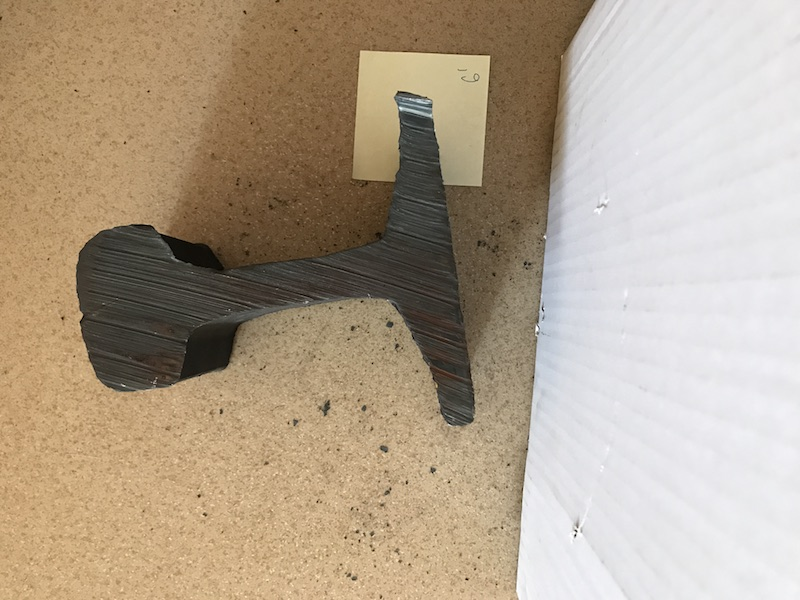
\includegraphics[width=0.45\textwidth]{images/good_before_preprocessing}}
     \qquad
     \subfloat[After thresholding]{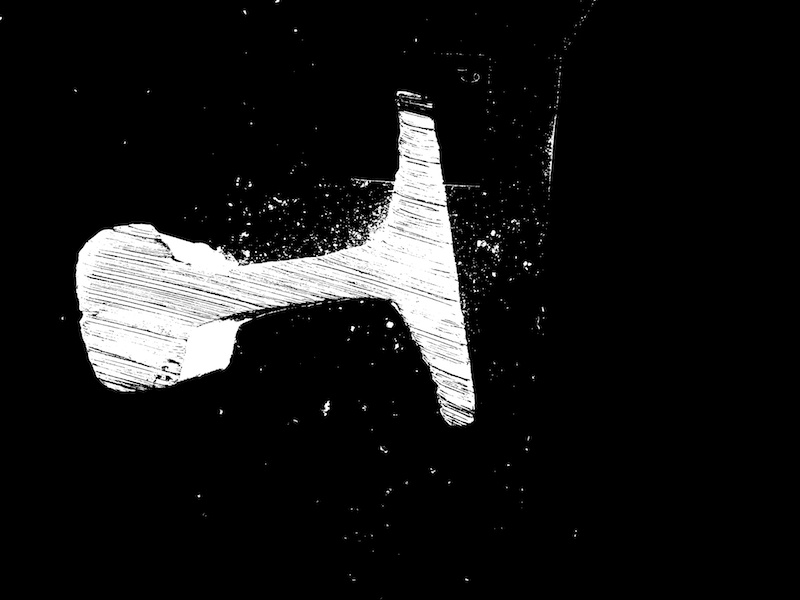
\includegraphics[width=0.45\textwidth]{images/good_after_thresholding}}
     \qquad
     \vfill
     \subfloat[After opening and blurring]{
\includegraphics[width=0.45\textwidth]{images/good_after_opening_and_blurring}}
     \qquad
     \subfloat[Shape detected]{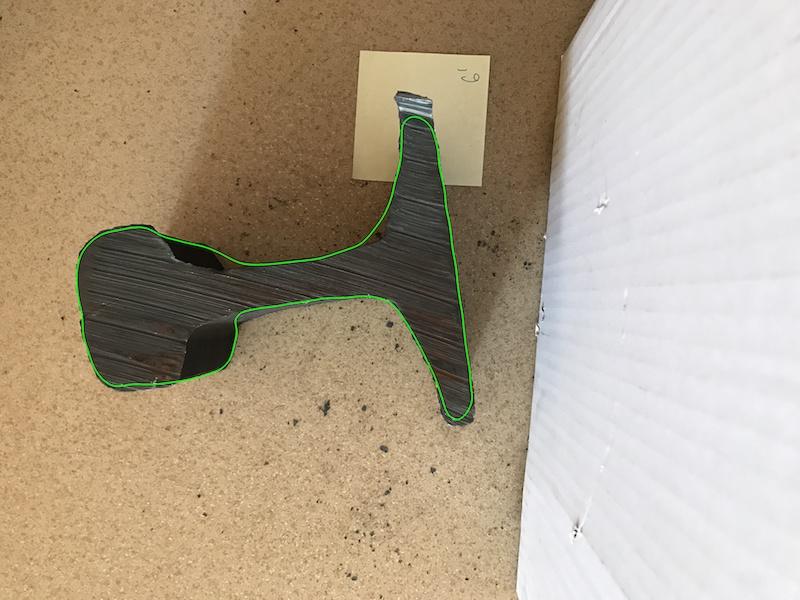
\includegraphics[width=0.45\textwidth]{images/good_after_preprocessing}}
     \caption{Stages of preprocessing - successful}
\end{figure}

\section{Image Processing}
\paragraph{}
Given that the main purpose of the thesis is the identification of foundry details, we can skip further contemplation of the preprocessing phase. The shape detection and extraction can be treated as a separate algorithm that needs to be developed and fine-tuned.
\paragraph{}
Assuming we have such an algorithm and thus a successful preprocessing phase, in the actual computing phase the input images contain only the surfaces of the splints (see figure \ref{fig:preprocessing_outputs}).

\begin{figure}[H]
     \centering
     \subfloat[]{\fbox{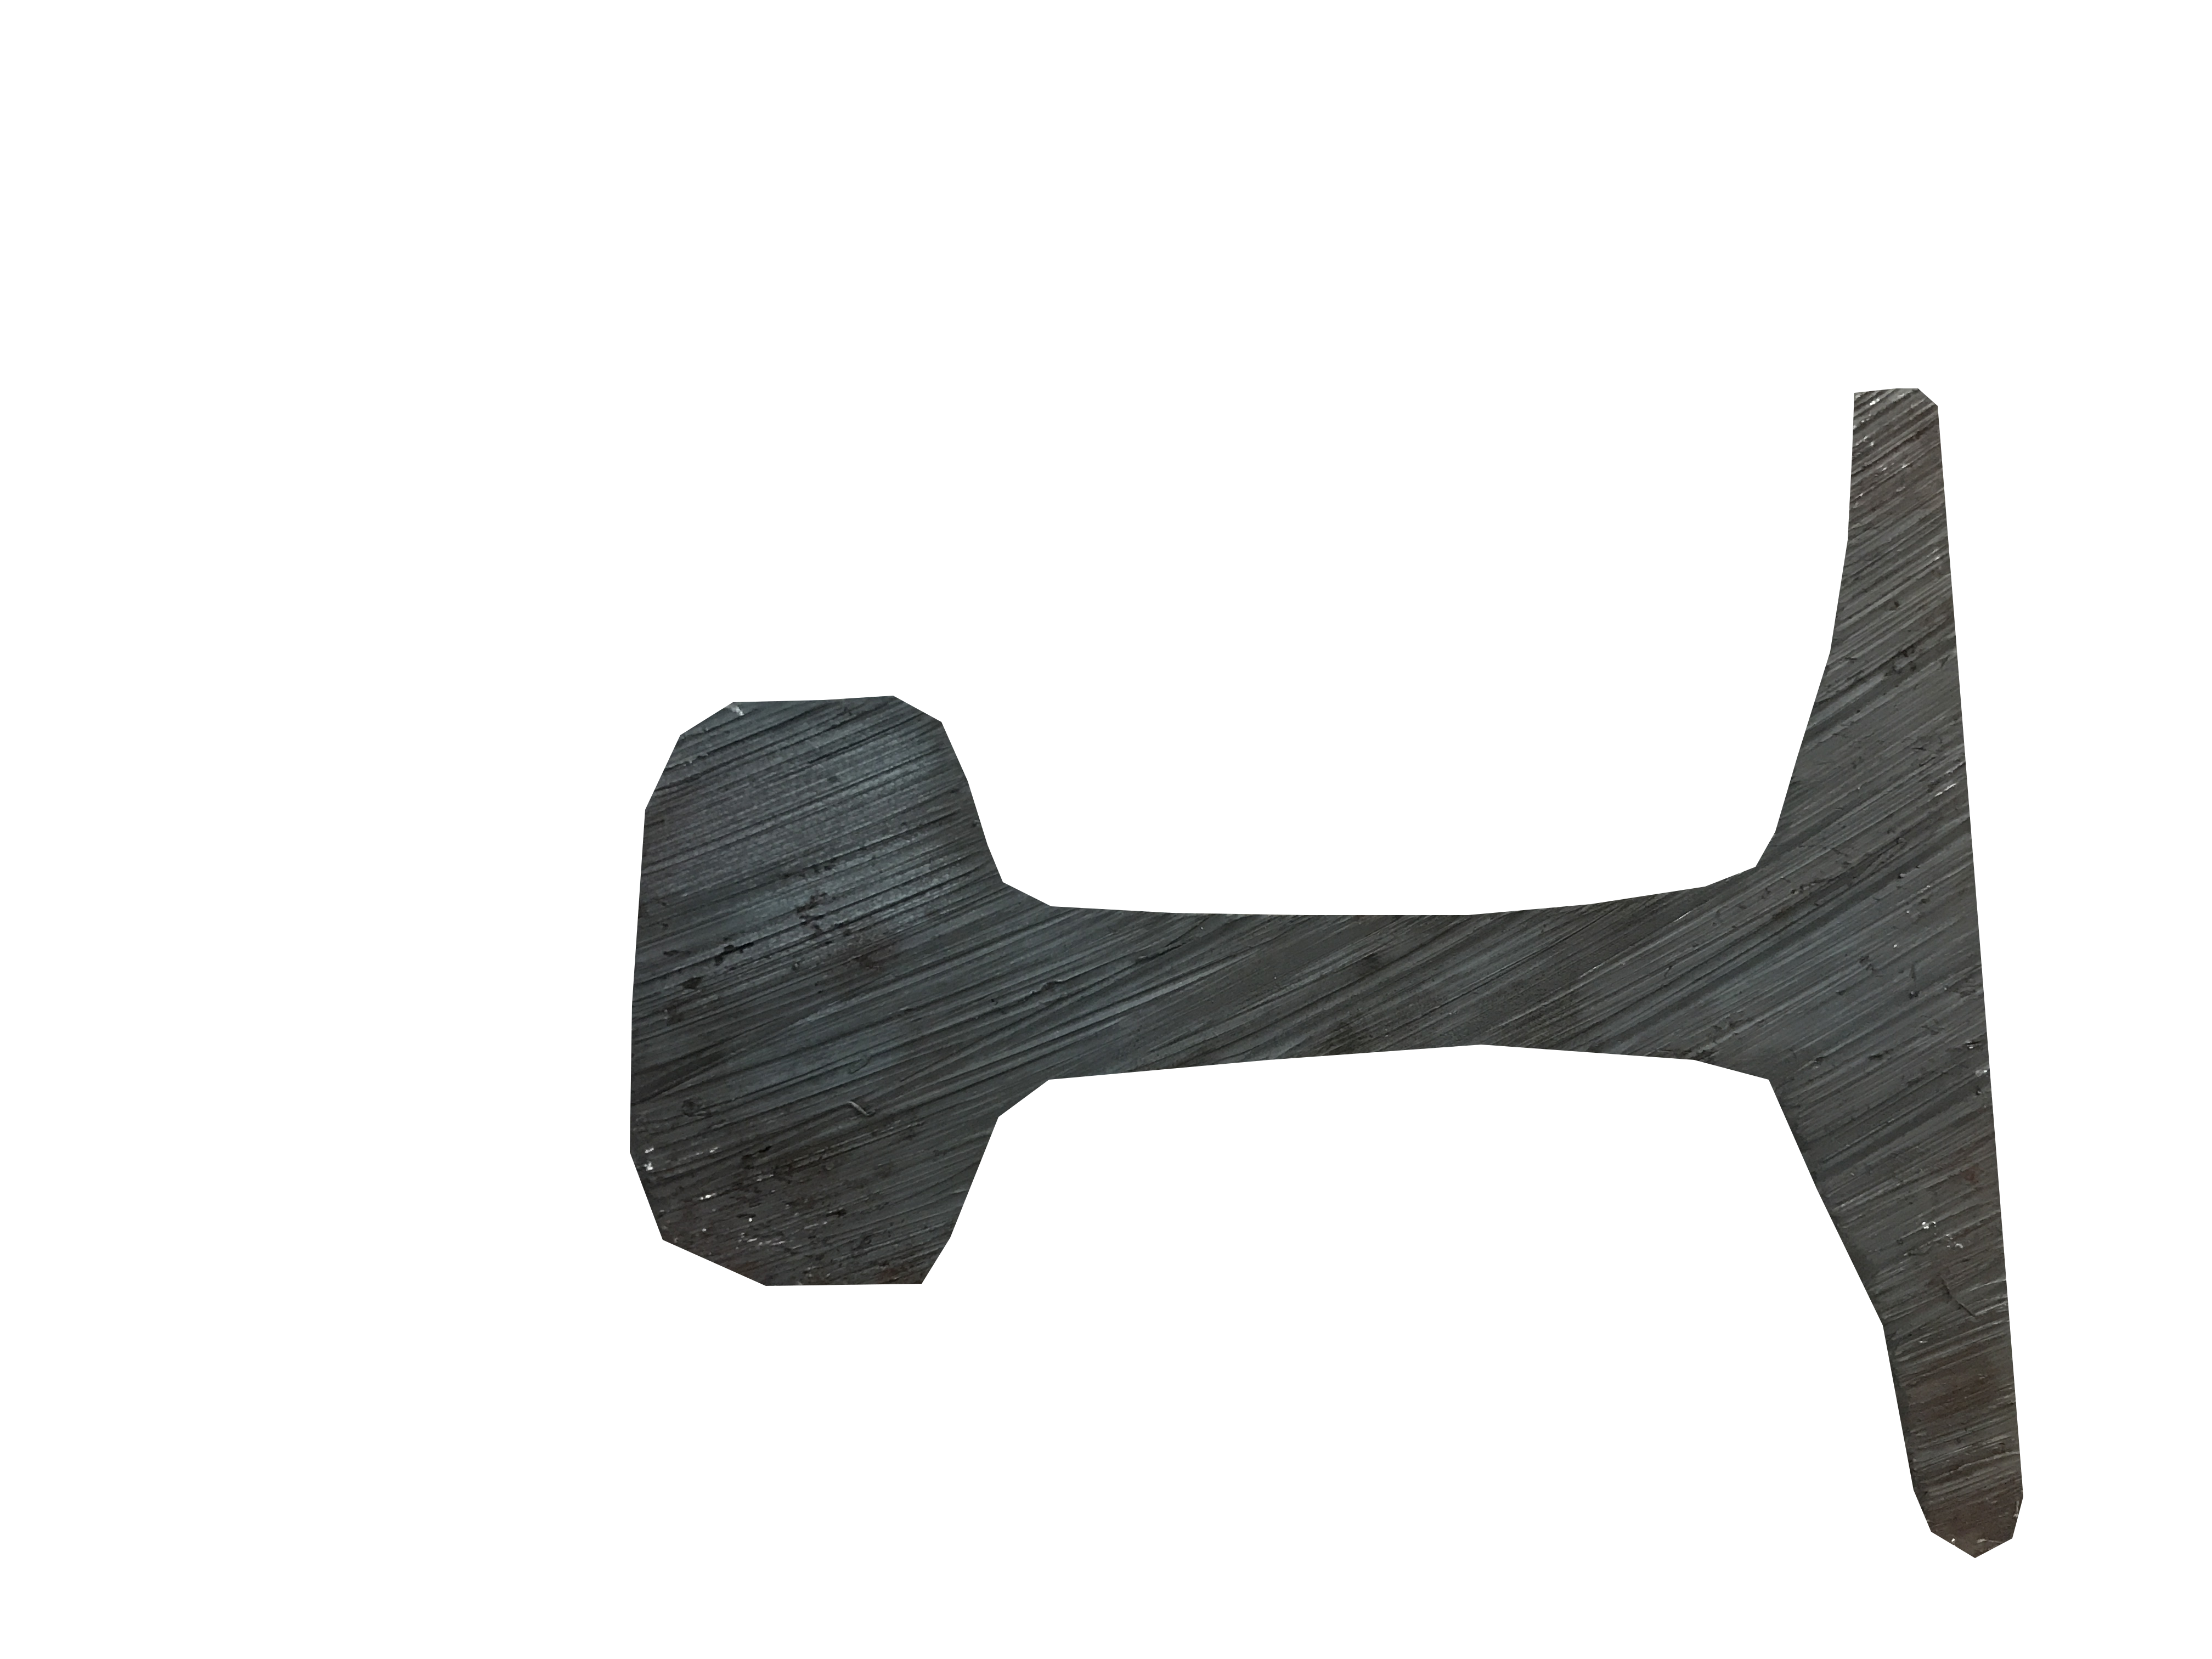
\includegraphics[width=0.45\textwidth]{images/preprocessed_1}}}
     \qquad
     \subfloat[]{\fbox{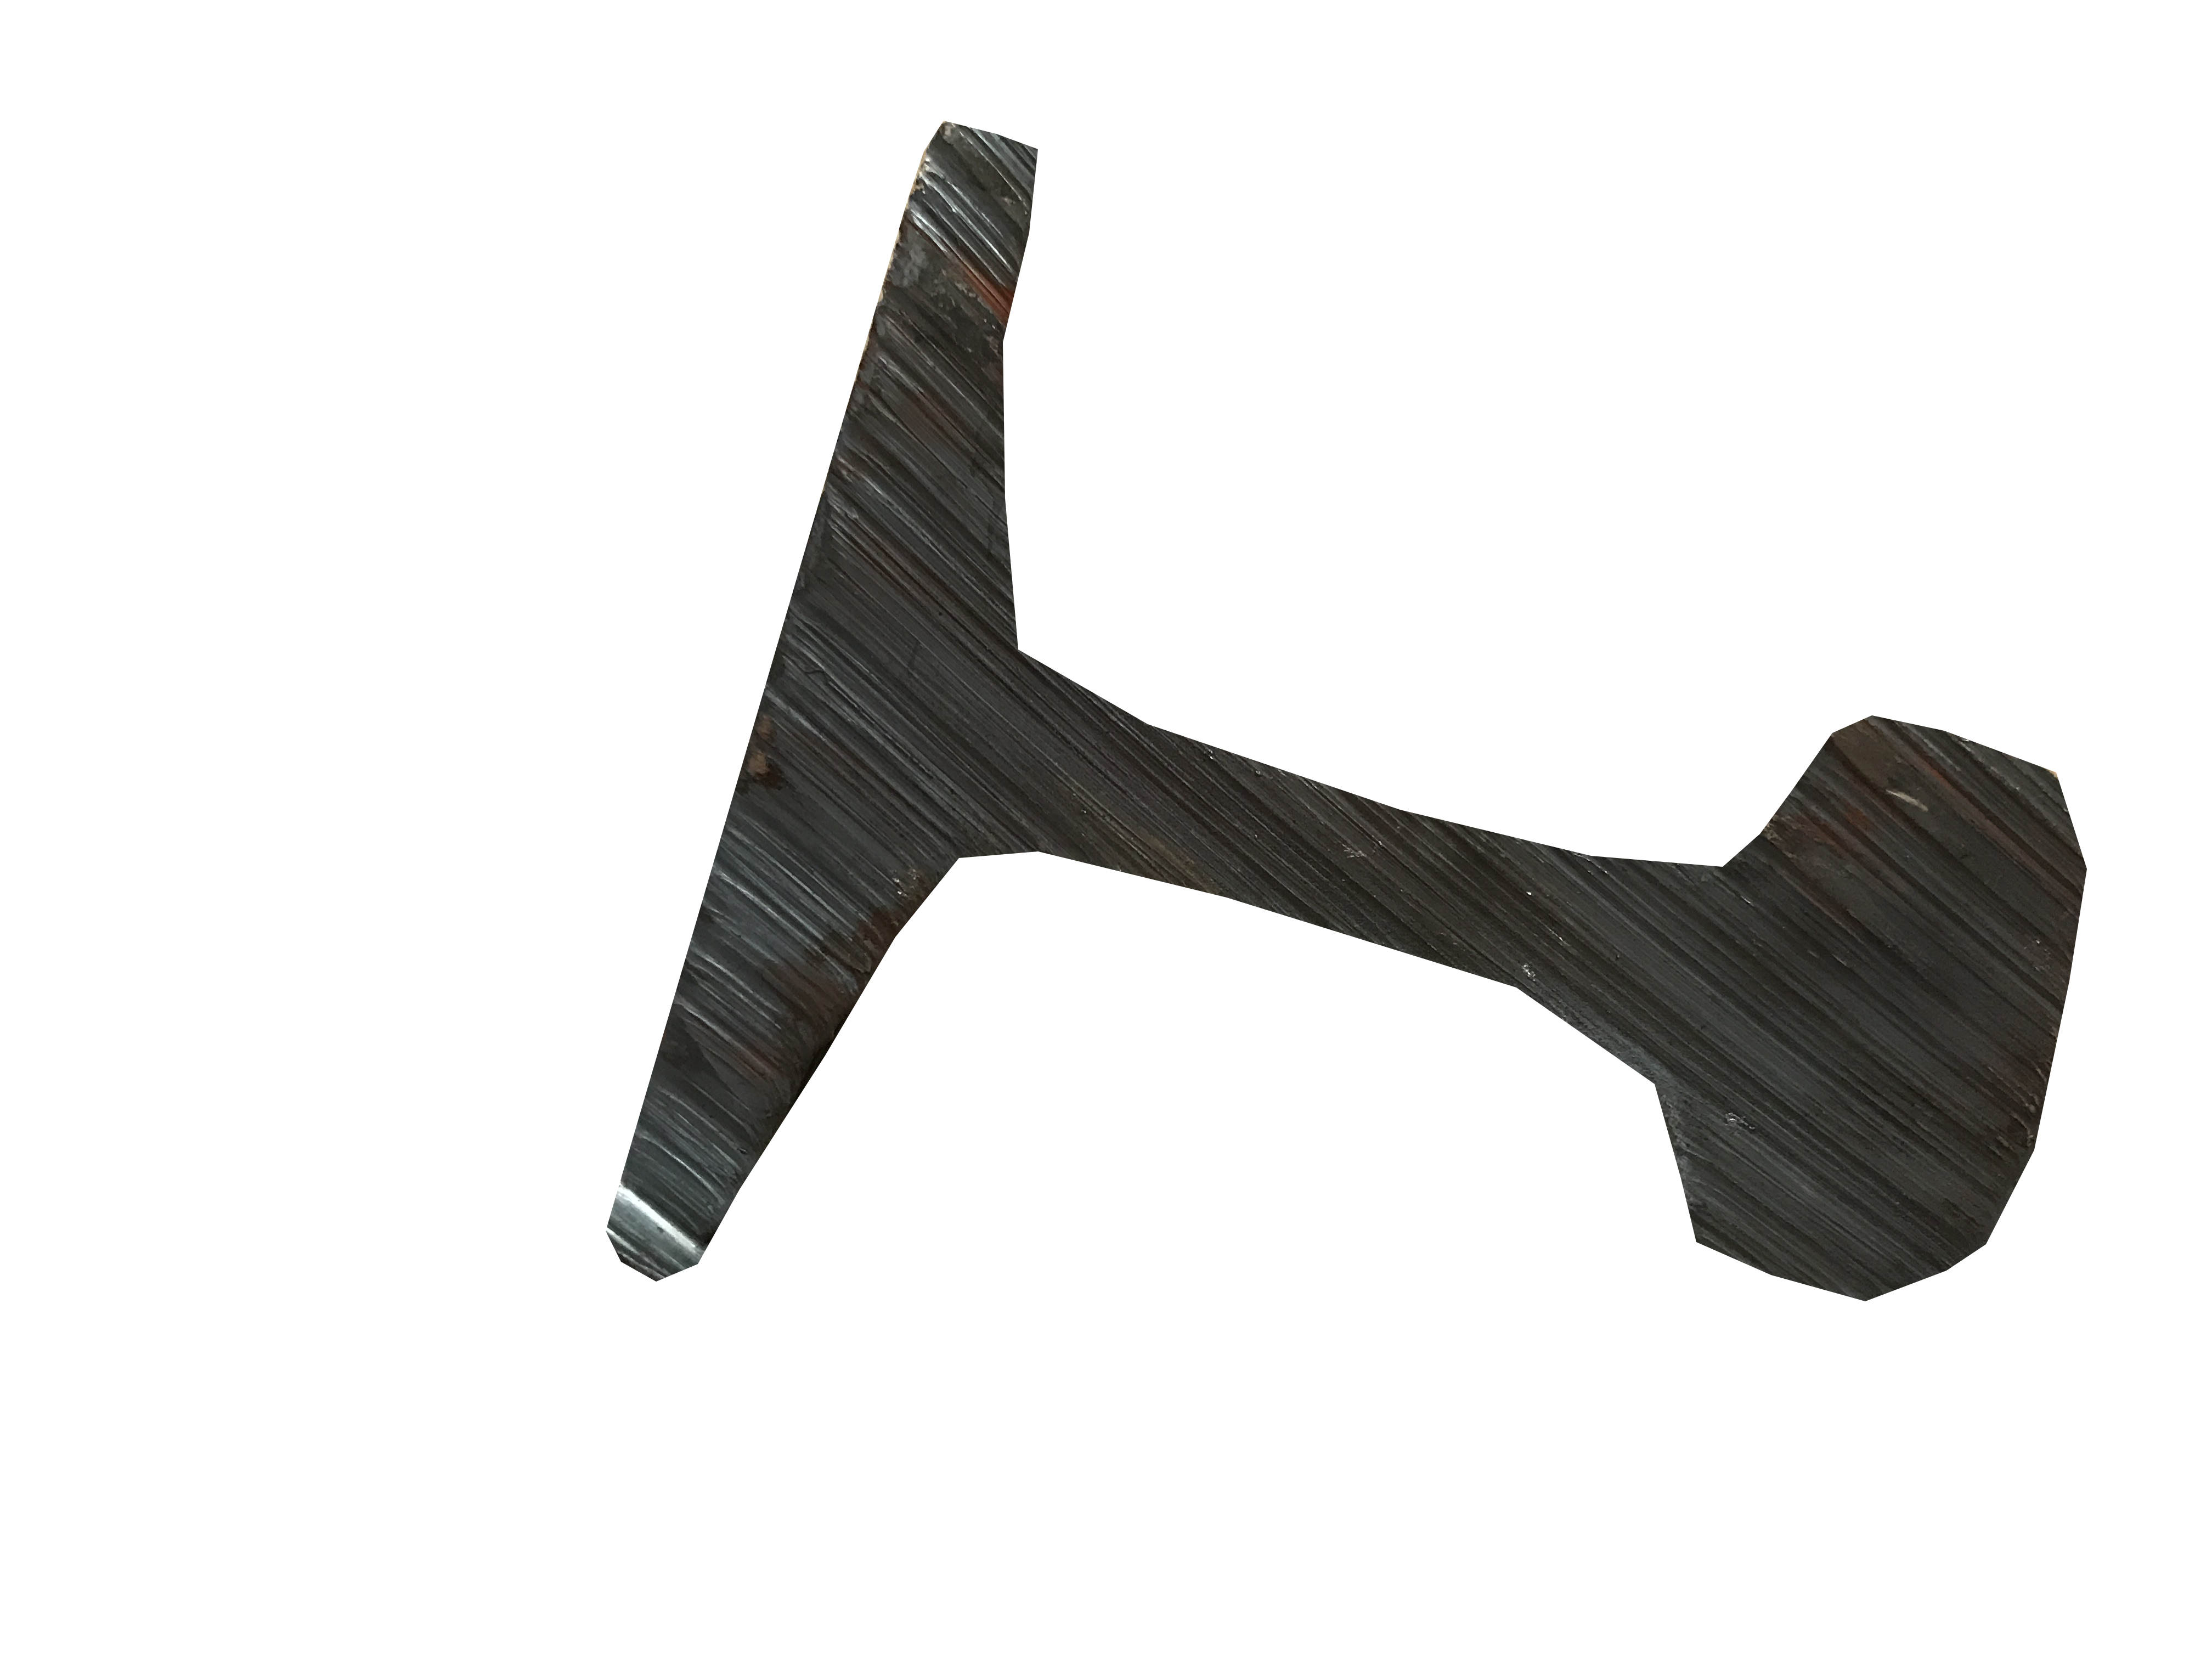
\includegraphics[width=0.45\textwidth]{images/preprocessed_2}}}
     \qquad
     \vfill
     \subfloat[]{\fbox{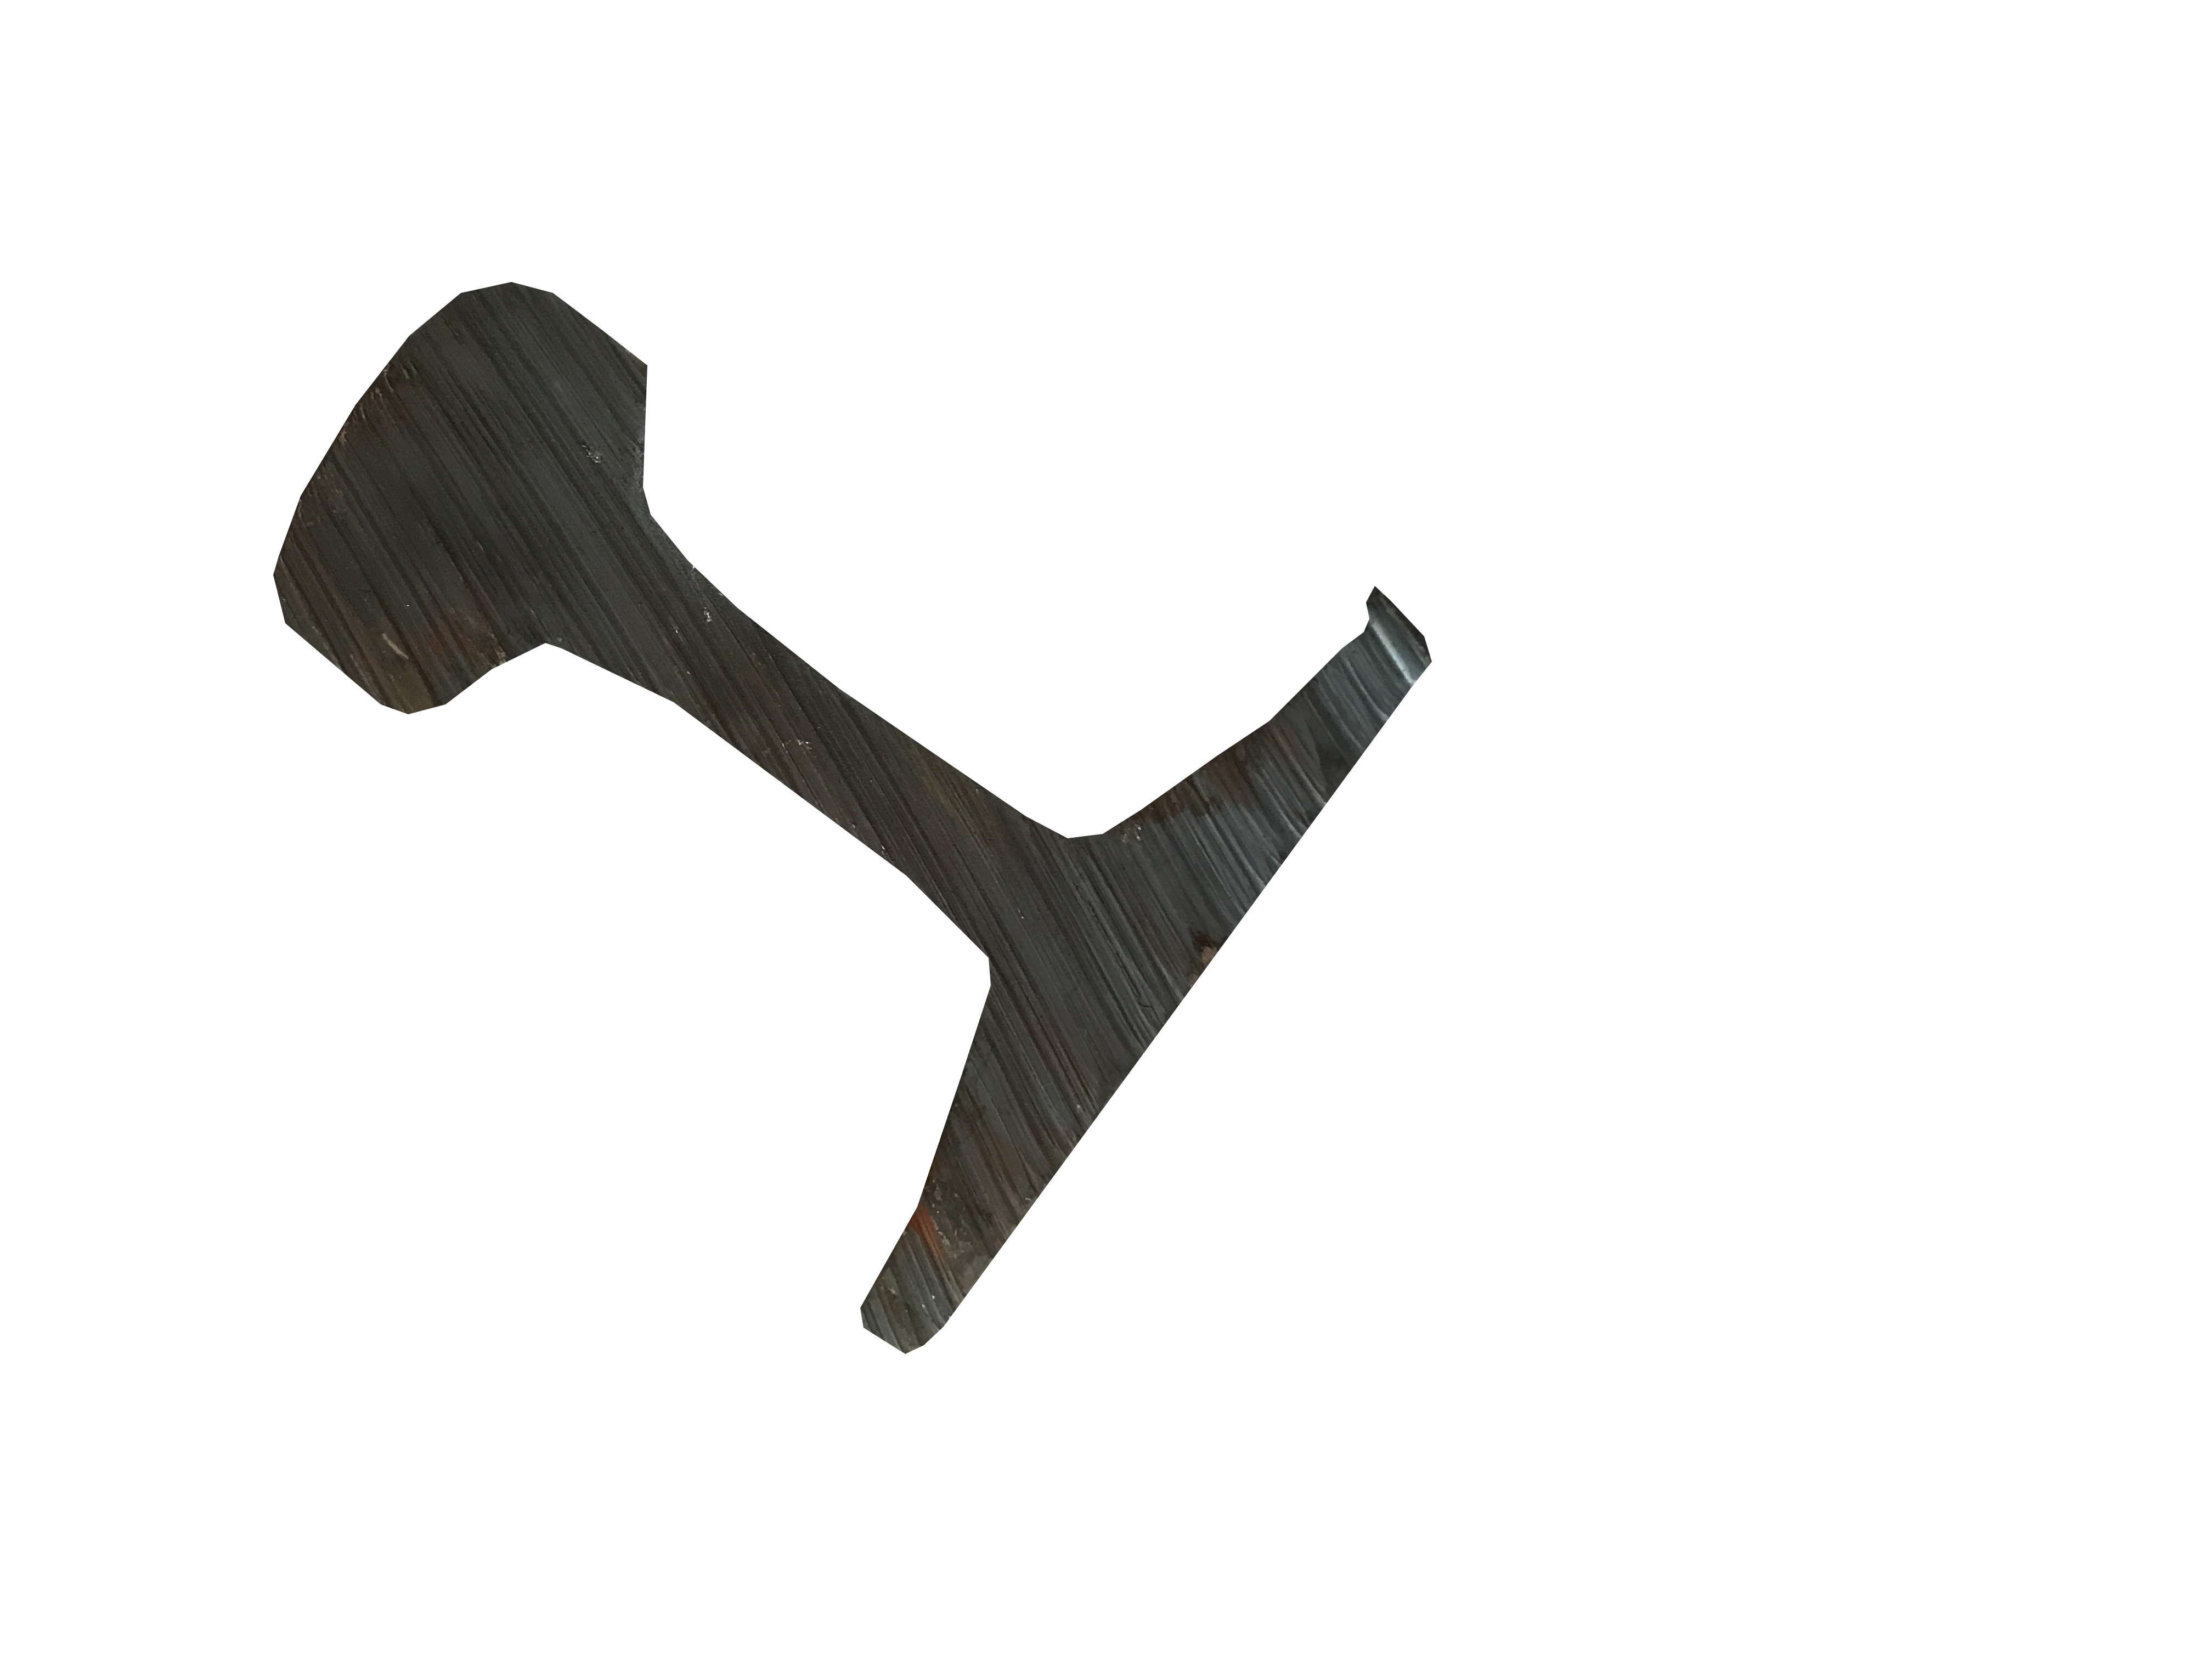
\includegraphics[width=0.45\textwidth]{images/preprocessed_3}}}
     \qquad
     \subfloat[]{\fbox{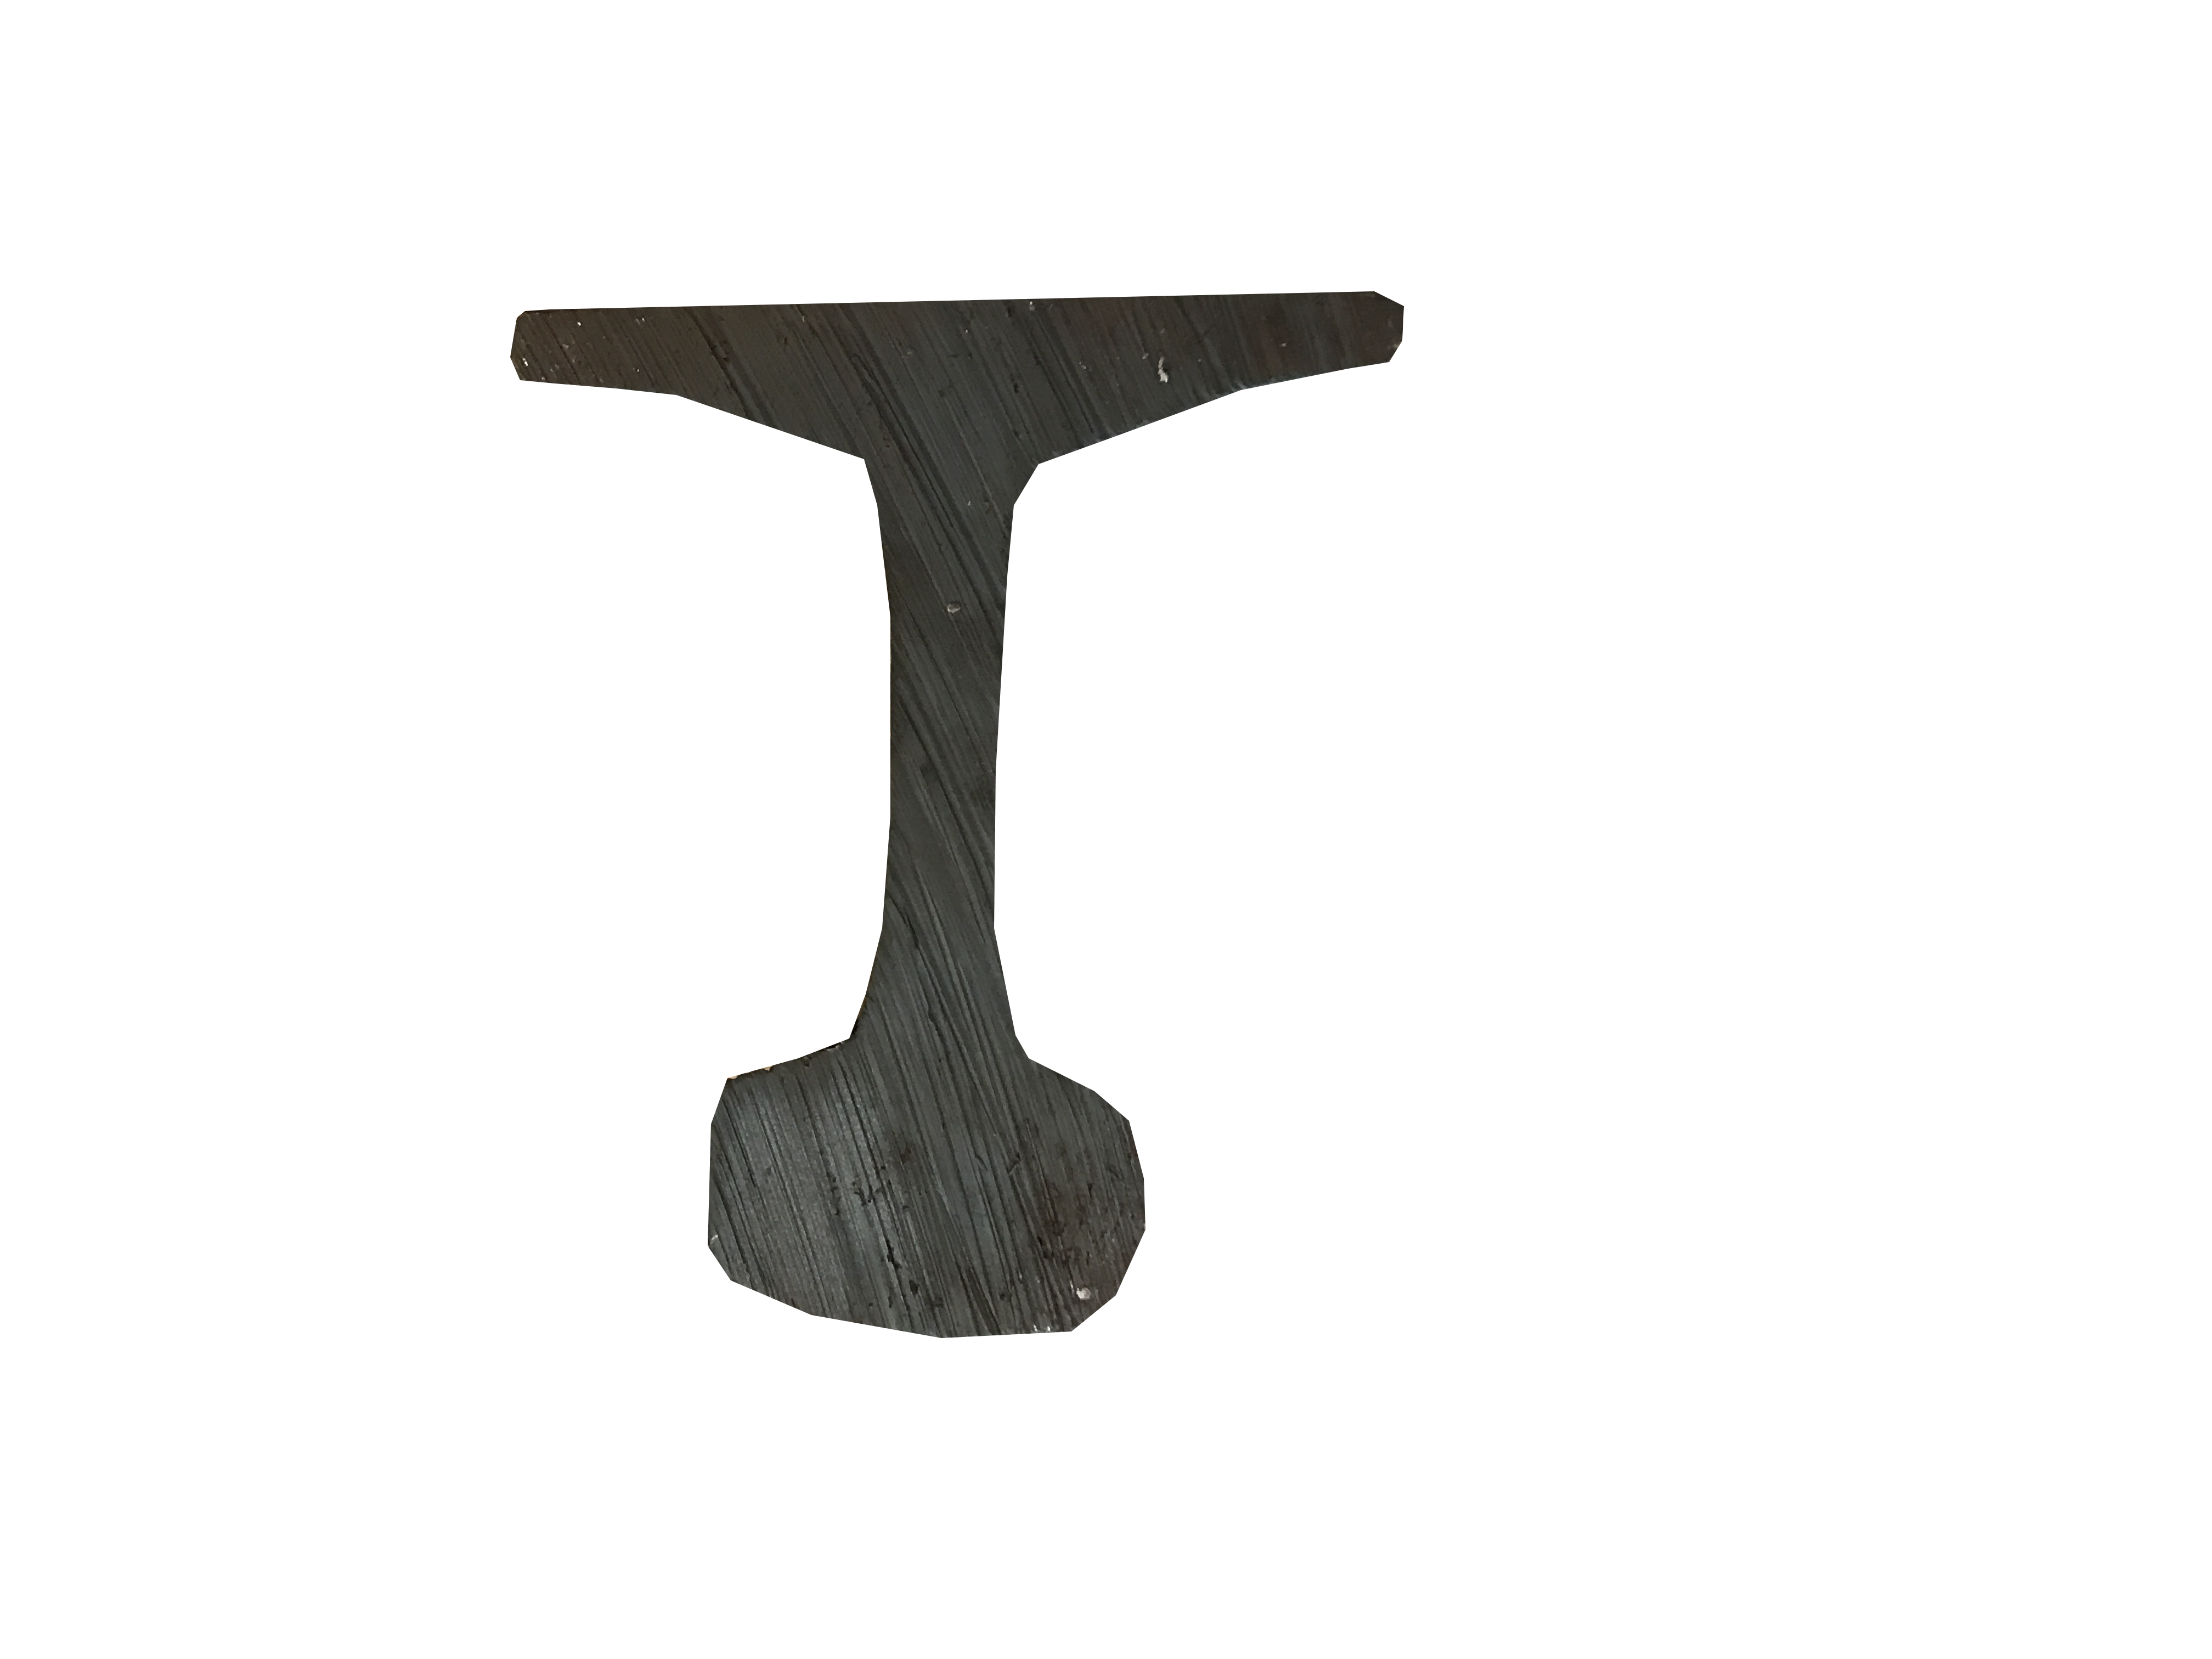
\includegraphics[width=0.45\textwidth]{images/preprocessed_4}}}
     \caption{Preprocessing outputs}
     \label{fig:preprocessing_outputs}
\end{figure}

\paragraph{}
In order to reduce complexity of the processing phase, a need to find some optimizations emerged. One of the solutions that was under investigation was to scale the image down - but it led to more noise being introduced and thus the comparison results being less accurate. Experiments and development of the processing algorithm showed that the most significant part for the comparison of barcodes lies in the upper half of the splint surface - the "ellipse-shaped" part of it. It is due to the fact that this area is the most stable across all of the images in terms of the barcode readability and consistency. This is why the lower part of the image is actually dropped altogether from the analysis.

\paragraph{}
Let us now look at the algorithm for comparing two images. 

\begin{algorithm}{\textbf{Comparing two preprocessed splint images}}
	\begin{spacing}{1.5}
	\begin{algorithmic}[1]
		\Function{compare}{$image1, image2$}
			\State $image1\_up \gets$ upper half from the $image1$
			\State $image2\_up \gets$ upper half from the $image2$
			
			\State $angle1 \gets \textbf{dominantAngle}(image1)$
			\State $angle2 \gets \textbf{dominantAngle}(image2)$
			
			\If{$\textbf{abs}(angle1 - angle2) > \textbf{THRESHOLD\_ANGLE}$}
				\State \textbf{return} FALSE
			\EndIf
			
			\State $rotated1 \gets \textbf{rotate}(image1\_up, angle1)$
			\State $rotated2 \gets \textbf{rotate}(image2\_up, angle2)$
			
			\State $result \gets \textbf{findMaxComparisonResult}(rotated1, rotated2)$
			\State \textbf{return} $result > \textbf{THRESHOLD\_COMPARISON}$
		\EndFunction
	\end{algorithmic}
	\end{spacing}
\end{algorithm}

\paragraph{}
Explanation

\begin{itemize}
	\item \textbf{dominantAngle(image)} - this function finds the most frequent angle amongst the lines that create the pattern. The image first undergoes Canny Edge detection, so line detection algorithm can later be used. It does so by utilising OpenCV's \textbf{HoughLinesP} function from which those angles can be computed, rounded and the dominant one is selected. The pseudocode and some explanation for this algorithm is provided later in this chapter.
	\item \textbf{rotate(image, angle)} - this function simply rotates the image by a given angle. It is used to point the lines that form the patter perpendicular to X-axis.
	\item \textbf{findMaxComparisonResult(image1, image2)} - this function is returning the final comparison result. In order to alleviate some differences in the dominant angle resulting in slightly different rotations, this function itself also does some minor rotations for first of the images and each such rotation is being compared with the second image. Maximum value of those comparisons is then returned as the final value.
\end{itemize}

\begin{algorithm}{\textbf{Comparing two preprocessed splint images}}
	\begin{spacing}{1.5}
	\begin{algorithmic}[1]
		\Function{dominantAngle}{$color\_image$}
			\State $equalized \gets \textbf{equalizeLight}(color\_image)$
			\State $gray \gets \textbf{cv2.cvtColor}(equalized)$
			\State $edges \gets \textbf{cv2.Canny}(gray)$
			\State $angles \gets []$
			\State $lines \gets \textbf{cv2.HoughLinesP}(edges)$
			\For{$line \gets lines$}
				\State $x1, y1, x2, y2 \gets line$
				\State $a \gets $ slope of $x1, y1, x2, y2$
				\State $angle \gets$ get angle for $slope$
				\State $angles.append(angle)$
			\EndFor
			\State $histogram \gets \textbf{np.histogram}(angles, bins=360, range=(0, 180))$
			\State $convolution \gets \textbf{np.convolve}(hist, \textbf{np.ones}(6))$
			\State \textbf{return} $\textbf{np.argmax}(convolution) / 2.0$
		\EndFunction
	\end{algorithmic}
	\end{spacing}
\end{algorithm}

\paragraph{}
In order to accommodate for some relic peaks, it is actually not the most frequently occurring angle but it is accumulatively taken within 3 degrees and only then the max is picked.

\begin{figure}[H]
     \centering
     \subfloat[Original input]{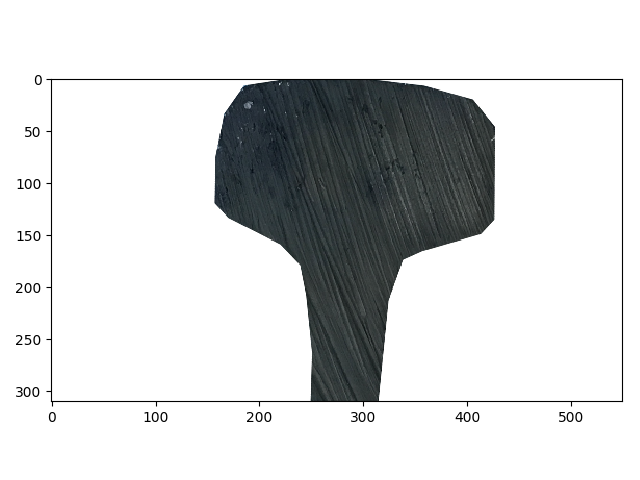
\includegraphics[width=0.75\textwidth]{images/up}}
     \vfill
     \subfloat[Rotated]{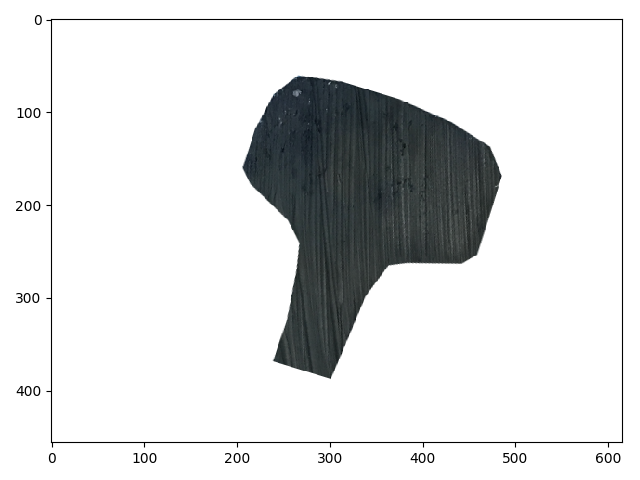
\includegraphics[width=0.75\textwidth]{images/rotated_up}}
     \caption{Rotation perpendicular to X-axis}
     \label{fig:image_rotation}
\end{figure}

\begin{figure}[H]
     \centering
     \subfloat[Pattern code]{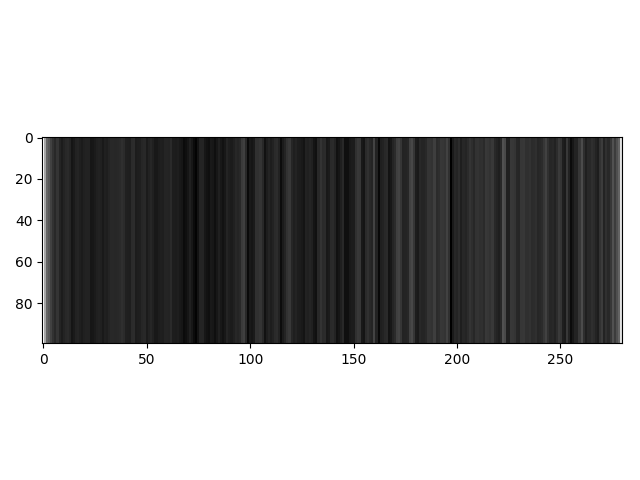
\includegraphics[width=0.75\textwidth]{images/rotated_up_code}}
     \vfill
     \subfloat[Corresponding histogram]{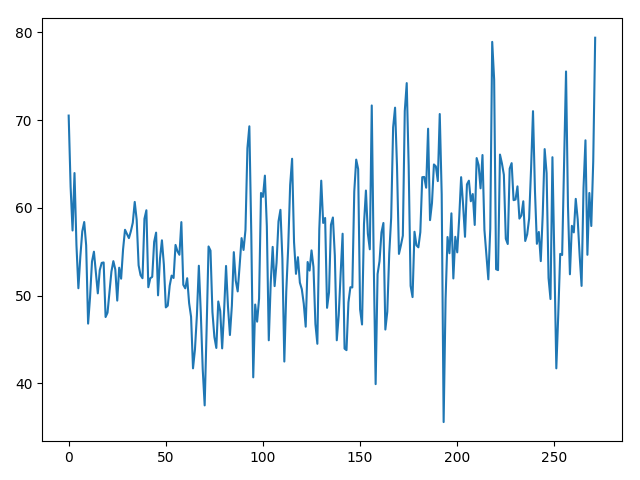
\includegraphics[width=0.75\textwidth]{images/rotated_up_hist}}
     \caption{Code and its' histogram}
     \label{fig:code_with_histogram}
\end{figure}

\paragraph{}
Figure \ref{fig:image_rotation} presents the already-extracted upper half of the splint surface before and after rotation. This procedure outputs an image, where the "barcode" lines are aligned perpendicular to the X-axis. After that, figure \ref{fig:code_with_histogram} shows the code that was read from the image (it actually is a single-row vector, only for graphing purposes that row is multiplied and we can see the code) and the histogram that corresponds to its grayscale values.

\paragraph{}
The whole process of mapping the splint image to a barcode (single-row vector) was to reduce the dimensionality of the task on hand. Now it was just a matter of finding a smart way to compare this vectors and assign them some similarity score. This is where the histogram that was computed on the earlier stages comes in handy. There are already known methods of comparing them and one that was performing well was chosen in the comparison algorithm implementation.

\paragraph{}
To actually compare two histograms $H_1$ and $H_2$ a metric $d(H_1, H_2)$ is to be chosen. The algorithm uses \textbf{correlation} (which is selected by using \textbf{CV\_HISTCMP\_CORREL} flag for OpenCV's \textit{compareHist} function). The metric is then defined as:
\begin{equation}
	d(H_1, H_2) = \frac{\sum_I(H_1(I) - \bar{H_1})(H_2(I) - \bar{H_2})}{\sqrt{\sum_I(H_1(I) - \bar{H_1})^2 \sum_I(H_2(I) - \bar{H_2})^2}}
\end{equation}
where:
\begin{equation}
	\bar{H_k} = \frac{1}{N} \sum_J H_k(J)
\end{equation}
and $N$ is the total number of bins in histogram.

\paragraph{}
The histograms that are obtained for two splint images may actually differ in sizes and for the aforementioned comparison method they need to be same-sized. That is why we take the shorter histogram and slide it over the longer one, do the comparison one offset at a time and take the highest from the output values.

\begin{algorithm}{\textbf{Histogram comparison}}
	\begin{spacing}{1.5}
	\begin{algorithmic}[1]
		\Function{compareHist}{$h1, h2$}	
			\If{$\textbf{length}(h1) == \textbf{length}(h2)$}
				\State \textbf{return} $cv2.compareHist(h1, h2, cv2.HISTCMP\_CORREL)$
			\ElsIf{$\textbf{length}(h1) > \textbf{length}(h2)$}
				\State \textbf{return} $\textbf{maxHistComparison}(h1, h2)$
			\Else
				\State \textbf{return} $\textbf{maxHistComparison}(h2, h1)$
			\EndIf
		\EndFunction
	\end{algorithmic}
	\end{spacing}
\end{algorithm}

\begin{algorithm}{\textbf{Histogram comparison - helper function}}
	\begin{spacing}{1.5}
	\begin{algorithmic}[1]
		\Function{maxHistComparison}{$longer, shorter$}	
			\State $\text{len\_shorter} \gets \textbf{length}(shorter)$
			\State $\text{diff} \gets \textbf{length}(longer) - \textbf{length}(shorter)$
			\State $\text{max\_result} \gets -1$
			\For{$\text{offset} \gets 0\ \textbf{to}\ \text{diff}$}
				\State $\text{result} \gets \textbf{compareHist}(longer[\text{offset : offset + len\_shorter}], shorter)$
				\State $\text{max\_result} \gets \textbf{max}(\text{max\_result, result})$
			\EndFor
			\State \textbf{return} $\text{max\_result}$
		\EndFunction
	\end{algorithmic}
	\end{spacing}
\end{algorithm}

\newpage
\paragraph{}
The final result of the comparison, as already mentioned before, takes into consideration some slight differences in the dominant angle detection (does so be applying some artificial rotations in the process) and also for the size of the code (because the smaller one is searched through the larger one). Such a result - the similarity score - is then simply compared to a threshold value. If this outcome is greater than that threshold we can say that both images represent splint with the same code, which in our case means it represents the same splint. Otherwise, we can say that those images represent two different splints.











